\subsection{Background}

\paragraph{}The MNIST dataset has long been regarded as a benchmark for evaluating machine learning 
algorithms on image recognition tasks. Comprising 70,000 grayscale images of handwritten digits 
(0-9), MNIST has served as a cornerstone for research in optical character recognition (OCR). Its 
simplicity, coupled with its real-world relevance, makes it a valuable dataset for testing new 
techniques and advancing the field of computer vision.

\paragraph{}With the increasing reliance on automation, the ability to accurately recognize handwritten digits 
has applications in diverse domains such as postal sorting, bank check processing, and document 
digitization. Traditional machine learning methods, such as k-Nearest Neighbors (k-NN) and Support 
Vector Machines (SVMs), have achieved moderate success on this dataset. However, the advent of deep 
learning, specifically Convolutional Neural Networks (CNNs), has revolutionized the accuracy and 
efficiency of image classification tasks.

\subsection{Objective}

\paragraph{}This project aims to develop and evaluate a Convolutional Neural Network (CNN) to 
classify handwritten digits from the MNIST dataset. CNNs, designed to mimic the visual processing 
mechanisms of the human brain, leverage their ability to learn spatial hierarchies of features 
directly from images, eliminating the need for manual feature extraction. The goal is to achieve 
high classification accuracy while demonstrating the advantages of CNNs over traditional methods.

\begin{figure}[H]
  \begin{center}
    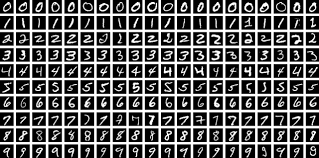
\includegraphics{img/introduction/mnist.png}
    \caption{Sample images from the MNIST dataset}
  \end{center}
\end{figure}
